\chapter{Discussion: Implications for Intercultural Communication Research}
\lhead{\textit{Discussion: Implications for Intercultural Communication Research}}

\textit{\textbf{Chapter Summary:} This final chapter discusses how the key research conclusions can be placed within intercultural communication research. It does this by focusing on three themes (i) methodological implications, (ii) the topic of the nature within ICC, and (iii) intercultural competence. Directions for further research are then discussed to conclude the dissertation.}
\newline

Chapter 2 outlined the historical evolution of intercultural communication as a field of study. The various turns in the discipline since the mid-twentieth century led us to a multilevel framework that accounted for the macro-context as well as the cognitive micro-context of communicative interactions. This framework was then applied to analyze real-word communication data. The stated research aim was to lay a conceptual groundwork for understanding ecological issues in the context of human culture and communication. This groundwork was summarized in the preceding chapter. 

This research question is relevant to corpus and applied linguistics, environmental communication, ecolinguistics, and related sub-fields. The research question also touches on intercultural philosophy. However, the aims and methods employed are rather unconventional when it comes to more applied intercultural communication research. That said, there are several insights more directly related to intercultural communication practice. This chapter discusses these insights, aiming to more explicitly place this research among intercultural communication literature and practice.

The chapter sections, and the intercultural communication questions they relate to, are as follows: 

\begin{itemize}

    \item \textit{Methodological Implications}: ICC is faced with the challenge of studying culture in an age when people have multiple identities. Based on the analyses in this dissertation, what are some possible departure points for ICC research? What are the prospects for corpus-based methods in intercultural communication research?

    \item \textit{Nature within ICC Research}: comparative intercultural research has been premised on dimensions of cultures (e.g. time orientation, power distance, individualism-collectivism) \citep{Hofstede2010a, House2004}. Can the natural world be considered a dimension of culture? How can the natural world be part of ICC scholarship?
    
    \item \textit{Intercultural Competence}: Does this research offer new insights into behaviours and communication styles that promote mutual understanding? 

    \item \textit{Directions for Further Research}: How could the questions raised in this dissertation be further pursued as part of an ICC research program? 
    
\end{itemize}

\section{Methodological Implications}

As alluded to in previous chapters, intercultural communication research faces considerable ``theoretical turbulence'' \citep{Poutiainen2014}. Quantitative and positivist approaches, exemplified in the work of \cite{Hofstede2010a} or \cite{House2004}, aim to objectively measure cultures. Interpretive approaches, by contrast, argue that cultures are better understood through qualitative methods. Critical theorists would challenge positivist methods on the basis that they omit analysis and deconstruction of social and political power. Theoretical turbulence inevitably leads to methodological turbulence, since how we study interculturality will depend on how we frame it conceptually.  

The multilevel framework used in this dissertation aims to strike a balance between interpretive and critical approaches. By isolating socio-economic and cultural analyses, the researcher is compelled to take both approaches (interpretive and critical) into account. Moreover, corpus methods lend themselves to quantitative research, albeit in a quite different manner than has been most common in ICC studies, namely the statistical interpretation of survey data as in \cite{Hofstede2010a} or \cite{House2004}. The methods in these latter studies are comparative across cultures, where culture is largely defined in terms of nation-state or geographic region. \cite{Hofstede2010a}, for instance, distinguishes cultures as Latin, African, East-Asian, North American, Germanic, and so on. 

This present dissertation departs from conventional ICC research and common notions of what constitutes intercultural communication. The analyses looked exclusively at communication in the English language. The artifacts and data emerge almost exclusively from Anglo-American culture with two of the three analyses geographically centred in the United States. Accordingly, one might question what is explicitly intercultural about the communication in the three analyses presented in this dissertation. 

There are two answers to this question. The first, and perhaps most obvious, is that modern nation states are a mosaic of cultures and identities. In the analysis of the Dakota Access Pipeline, for instance, we saw references to indigenous, African American, and white Christian identities. It is imperative for intercultural communication research to account for the complex ways in which multiple identities combine, both at the societal level as well as hybrid identities within individuals. A second, perhaps less obvious reason that the preceding analyses connect with intercultural communication, is the conviction that intracultural or intergroup communication issues need to be looked at alongside the intercultural. The reason for close alignment with intergroup communication relates to identifying the variables and context of intercultural encounters.

\subsection{Variables \& Context}

\cite{Gudykunst2001} explains how intercultural communication is one subtype of intergroup communication. As was apparent in various analyses in this dissertation, contemporary communicative misunderstandings occur along the intersecting lines of class, region, ideology, profession, etc. This is not to suggest all such communication be considered intercultural; rather, these factors are crucial in understanding the context of intercultural communication. As \cite{Barnett2001} explain:

\begin{quote}
Context is a crucial concern for intercultural research. It includes economic, political, educational, and religious factors (Parsons, 1968), as well as the family and the media, society's level of technology, and society's infrastructure. Knowledge of the factors influencing the process of intercultural interaction is important to specify the relationship among intercultural variables. (283) 
\end{quote}

The methodological implication is that we do not begin by assuming that the intercultural dimension is the primary and only source of misunderstanding. In intercultural communication, cultural identities are often the starting and end points of analysis. The relevancy of these categories in each interaction is often not taken into account \citep{Nishizaka1999,Nishizaka1995}. As a result, some intercultural approaches might be criticised for failing to reflect the complexities of everyday, intergroup interactions \citep{Frame2014}.

A multilevel methodology specifies the context by deliberately omitting assumptions of cultural identity. In other words, the researcher does not assume that misunderstandings are due to cultural differences. By bracketing the socio-economic and cognitive levels, the researcher is considering a range of factors that may lead to misunderstanding. The ecological level likewise considers physical environment, infrastructure, and technology. Consequently, when the intercultural factors do come into play they can be more precisely identified and any misunderstandings understood in a wider context. 

Consider the analysis of GM seed discourse in Chapter 3. The starting point for this analysis is not communication from different cultural groups. We begin with the communication itself and identify many sources of misunderstanding including communities of practice, economic inequality, and cognitive frames. The intercultural aspects of this debate are then embedded within these many factors. By first identifying these factors, intercultural aspects could then be specified, such as differences in connotative meanings, symbolism, and time orientation.

The multilevel discourse approach begins by looking at the richness and variety of communication itself. \cite{Dacheux} argues ICC scholars have often focused on the intercultural side of the equation and communication has been reduced to transfer of messages. This reduction might lead to simplistic assumptions about overcoming differences, whereby mutual understanding is a matter of adopting behaviours and styles that overcome otherwise mutually intelligible, transparent messages. The conceptual framework proposed in the previous chapter rebukes the notion that human communication can be reduced to information transfer. In multilevel discourse analysis, the communication itself is considered from multiple angles before intercultural factors even come into play. 

\subsection{ICC \& the Crisis of Globalization}

Another reason for a multilevel, intergroup approach relates to contemporary trends of globalization. A common narrative is that globalization has increased linkages among different cultural groups and has facilitated cross-border communication. In terms of a structural model of intercultural communication \citep{Barnett2001,Barnett2005}, the bridges (points a and b in Figure 7.1) and liaisons (point c) that exist between groups have become more numerous and their communicative exchanges more frequent. Similarly, an increase in the number and variety of mass media outlets has created more opportunities for transmission of cultural information within and between groups (Media A and Media B in Figure 7.1). One could make a similar argument for international organizations, since the numbers of both government and non-governmental organizations have increased in recent decades \cite[][15, citing data from www.uia.be]{Marshall2011}. From this structural theoretical standpoint, one might optimistically argue that globalization promotes intercultural communication by reducing uncertainty and allowing people to interpret and evaluate intercultural encounters more effectively \citep{Barnett2001}.

However, the optimistic argument is countered by what some have described as a crisis of globalization. Offshoring of jobs, trade deficits, migration, and inequality have led to opposition to globalization \citep{Cerna2015,Martin2018}. The rise of nationalism and populism in Europe and the Anglosphere \citep{Bieber2018, Bonikowski2019} is often attributed to a growing malaise with the globalization model that has been adopted since roughly the 1970s. 

It is incumbent on ICC researchers to understand this backlash and how it impacts intercultural interactions. There is little doubt that the decline of trust in media and institutions \citep{Lenard2005} changes the types of linkages we see in the structural model (Figure 7.1). Moreover, it is also possible that media and institutional actors perpetuate bias, stereotype, or other frames that run counter to effective intercultural communication. Accordingly, the critical analysis of socio-economic discourse, as well as cognitive structures such as ideologies and frames, are integral to ICC research.

\begin{figure}[H]
\centering
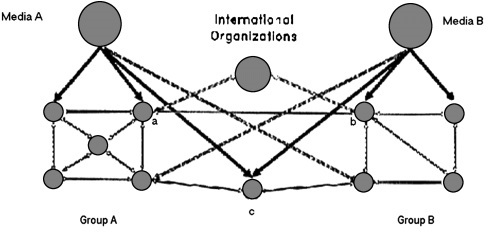
\includegraphics[width=10cm]{Figures/structuralmodel.jpg}
\caption{Structural Model of intercultural communication \citep{Barnett2005}}
\label{fig:figure1}
\end{figure}

In each of the three corpus analyses, we see examples of how global institutions and media shape the intercultural context. In the GM seed debate, a key theme is the dominance of global corporations and, in particular, the patent rights that have been granted through waves of international trade agreements and accompanying legislation. In the pipeline and mining debates, we consider the role of media in advancing stereotypes and contributing to in-group/out-group perceptions. In some cases, the presence of international institutions is used to label critics and environmentalists as outsiders who have little direct concern for the local community. 

To summarize, while conventional structural models suggest increased globalization will facilitate and ease intercultural encounters, contemporary reactions against globalization question this assumption. A multilevel discourse approach allows the researcher to carefully consider challenges globalization and mass media pose to effective intercultural communication.   

\subsection{The Role of Corpus-Based Methods}

A final methodological implication to consider is the role of corpus-based methods in intercultural research. Using secondary, corpus data runs counter to much ICC research given that many scholars in the field have limited intercultural communication to face-to-face interactions \cite[179]{Gudykunst2001}. However, in light of advances of globalization and information technology, we can consider that most intercultural interactions are now mediated by electronic devices, social media, and other technologies. Corpus methods allow for the systematic study of these interactions. Moreover, multimodal and audio-visual data permit the study of face-to-face interactions via corpus methods. However, it may be the case that corpus methods are not the entirety of an intercultural analysis. For instance, corpus data might be used to identify the context of intercultural communication, while the communicative interactions themselves are investigated through more direct methods and primary sources. 

The three corpora in this dissertation are a testament to the variety of topics and aspects of human communication that can be studied. Each corpus is quite distinct in terms of its contents as well as the dimensions of human communication contained within. The volume of data on the World Wide Web allows for the creation of specialized corpora. The data then provide a window into regions of language and communication that would otherwise be difficult to study had other data sources been used. That said, drawbacks of internet data must be kept in mind. When data is distributed via commercial search engine algorithms, issues of diversity, bias, and representativeness must be carefully considered. Given the plethora of search engine optimization and advertising copy, one must be aware of how the ``discourse of advertising'' \citep[99]{CurtisCollins2019} might overshadow authentic communication.

\section{Nature within ICC Research}

This dissertation has implications for how the natural world is approached in ICC research. While the previous chapter outlined conceptual principles along these lines, it remains unclear how these principles can be integrated into the main currents of intercultural communication research. This section will discuss the theme further, this time with more explicit reference to ICC literature.  

Part of the motivation for this dissertation is that ecology has not been a common theme in ICC research. This is not to say it has been entirely absent; rather, the topic is in need of a more firm grounding in the discipline. Where it has been factored into ICC research, nature has often been considered as a dimension of culture. In their \textit{Cultural Orientation Framework}, \cite{Kluckhohn1961} include ``orientation'' to the environment as one of six dimensions with which a society can be categorized. These authors identify subjugation, harmony, and mastery as culturally variable orientations to nature. Even if not assigned its own dimension, nature also falls under other categories. For instance, protection of the environment is considered under ``Universalism'' as a value priority with which Schwartz and colleagues compare countries \citep{Sagiv2000}. In the more recent \textit{Globe Study} \citep{House2004}, concern for the natural world could be considered part of the ``Future Orientation,'' one of the nine dimensions of cultural variability.

\subsection{Interpretive \& Critical Scholarship}

Previous studies have often approached orientation to nature as a statistical variable. The studies mentioned above, for example, use survey data as well as interviews to place different cultures on a relative scale. By contrast, the multilevel framework, together with conceptual principles proposed in the previous chapter, asks us to take a different methodological approach to nature than has been commonly observed in ICC research. Rather than viewing nature as among a handful of horizontal cultural variables, a multilevel approach hierarchically organizes the variables (as levels) from the macro to micro context. The ecological context is the macro level and is thus a starting point for understanding human communication. Nature and the environment form nothing less than semiotic context of human culture and communication. The environment is thus no longer one cultural variable among others, but analysis of human communication begins at the ecological level. The ecological level might focus on specific ecological themes and issues (as is the case in this dissertation), but could also include physical location, infrastructure, technology, soundscape, and other precursors to human communication.  

Based on the observations in this dissertation, we can conclude that the role of nature in communication and culture is too nuanced and complex to treat it as a quantitatively measured category. Qualitative, interpretive work is necessary before making generalizations about the meaning of nature for particular groups and cultures. Moreover, when collecting data through interviews and surveys, scholars need to be weary of \citeauthor{Beattie2016}'s (\citeyear{Beattie2016}) observation that there is a difference between what people explicitly say and how they feel about environmental issues. This observation is supported by the nonverbal study in Chapter 5, where we see how feelings and emotions associated with place and environment are often best understood through nonverbal, cognitive level analysis. Alongside primary sources (which may include interviews and surveys), multimodal corpus data of real communication events may be necessary to capture implicit feelings and attitudes.

With respect to critical approaches, this dissertation points to the importance of the analysis of political and economic dimensions of environmental issues and how these intersect with culture. Environmental and natural resource issues lie at the core of livelihoods and political/economic power. Alongside interpretive approaches, there is a need for the critical analysis of ecological-related communication. In each of the three analyses in this dissertation, the economic aspect was arguably the most contentious and gave rise to the strongest emotions. Critical approaches are needed to consider how culture is constructed in environmental discourse and how these constructions benefit certain interests.    

\subsection{Environmental Movements as Intercultural Spaces}

ICC scholarship is concerned with forums and spaces in which intercultural encounters take place. These forums and spaces are many and are evolving rapidly in global, technological society. At the same time, spaces for free, authentic communication are under threat. In line with critical analysis, we can consider that many communicative spaces are mediated and controlled by private interests. Social media, mobile networks, the built environment, etc., are most often owned and managed by corporate interests. One might question, therefore, where genuine intercultural encounters can take place.

In the previous chapter, the idea of the public sphere was introduced as precondition for deliberation. Specifically, it is proposed that the public sphere is a requirement for intercultural communication. Of particular interest for intercultural scholarship is how environmental protest movements are \textit{spaces of appearance} that reestablish the public sphere in societies where discursive spaces have been largely privatised. \cite*{Arendt1958a} describes space of appearance as ``the space where I appear to others as others appear to me, where men exist not merely like other living or inanimate things but make their appearance explicitly'' (198). The space of appearance is a precondition for the public sphere insofar as it ``precedes all formal constitution of the public realm and the various forms of government'' (199).

The notion of public sphere is particularly important in understanding communication related to the Dakota Access Pipeline. As discussed in Chapter 4, discourses in this corpus indicate a turning away form, and critique of, prevailing social institutions. The communication of pipeline opponents might be understood as an attempt to form alternative ``discursive spaces'' \citep[61]{Hauser1999a}. When peaceful pipeline demonstrators set up encampments in North Dakota, they were creating a discursive space. This can be understood as an establishment of the public sphere, after more official mechanisms (political, legal, media, etc.) were deemed futile. The socio-economic level of analysis in Chapter 4 discusses the closing off or denial of the public sphere. Quotes reveal how the pipeline protesters re-created the public sphere through a \textit{space of appearance}. 

Certain statements of protestors refer to a lack of voice and representation. The closing off of the public sphere, discussed in the socio-economic level of analysis, is expressed in the following statements:   

\begin{footnotesize}
\begin{itemize}
\item[] \texttt{We don't ever hear the narrative of indigenous people. We hear people writing our narratives for us.\newline 
\textit{-Eryn Wise, Council communications director}}
\newline
\item[] \texttt{It's just been escalating to that point where we have to use our phones to just show our side of our story. \newline 
\textit{-E'sha Hoferer, protester}}
\end{itemize}
\end{footnotesize} 

The denial of the public sphere experienced by protestors results in a sense of distance or alienation from social/institutional structures (i.e. civilization). As \cite*{Arendt1958a} states, ``alienation is the atrophy of the space of appearance'' (209). In other words, as alienation in a society grows, the space of appearance declines, and vice versa.

The protest site can be seen as the reestablishment of a place of appearance for those who felt it had been denied in the wider society. In Spring 2016, Standing Rock Sioux elder LaDonna Brave Bull Allard established a camp both as a centre of resistance to the pipeline and as a defense of sovereignty. By the summer, the camp had grown to thousands of people. Those at the camp referred to themselves as ``Water Protectors.'' In light of the negative connotations of ``protester'' (as discussed in the cognitive-level of analysis), the ``Water Protectors'' moniker can be seen as a way to re-frame how pipelines opponents are perceived and understood. 

To conclude, this dissertation calls for a reconsideration of the topic of the natural world within ICC research. Through both interpretive and critical approaches, the natural world can be given a central place in the discipline. At a more practical level, debates about infrastructure and natural resources are important intercultural spaces where expressions of identity take place in the public sphere. 

\section{Intercultural Competence}

In response to the three analyses in this dissertation, one might ask how these or similar misunderstandings could be overcome. In other words, are there principles or best practices that would enable mutual understanding in the context of environmental and resource issues? The premise of this question is that improved, more effective communication is possible on the part of various individuals and groups involved in these debates. In this section we consider this question by way of the concept \textit{intercultural competence}. In the discussion that follows, the concept of intercultural competence is seen as helpful but also in need of reconsideration. It is helpful in that there are principles of intercultural competence that are crucial in these contexts. However, we also argue that some principles and normative underpinnings of intercultural competence may need to be reconsidered in light of environmental issues. 

In short, we argue that many competence models, particularly those employed in stakeholder and public relations, have premises and underpinnings which do not transfer well to communication about ecological issues. There has been a recognition of the need for ICC research and models which are distinct to professional disciplines, notably medicine and education. In the same way, this section argues for ICC to be investigated more specifically in the domain of natural resources and ecology.       

\subsection{Cognitive Complexity \& Intercultural Competence}

Intercultural competence is a term to describe ``appropriate and effective communication and behavior in intercultural situations'' \cite[xi]{Deardorff2009}.  Competent communication has referred to an ability to identify and obtain goals, predict the behaviors and responses of the other communicator, choose effective communication strategies, and so on. It entails an understanding of acceptable behavior and meeting expectations and demands of situations \citep[209]{Wiseman2001}. A definition of intercultural competence that is consistent with the intergroup/intercultural concepts of this dissertation is that of \cite*{Spitzberg2009}: 

\begin{quote}
 the appropriate and effective management of interaction between people who, to some degree or another, represent different or divergent affective, cognitive, and behavioral orientations to the world. (7)   
\end{quote}


Various characteristics and behaviors of intercultural competence have been developed by ICC scholars as well as in related fields such as communication, psychology, foreign language, and management studies \cite[53-78]{Spencer-Oatey2009}. This includes research in applied linguistics and discourse studies which address problematic communication (ibid, 65). Research on intercultural competence has generally found that it results from a combination of personal capacities (e.g. flexibility, language skills, open-mindedness) and contextual factors (e.g. shared goals, perceptions) \citep{Arasaratnam}. 

\cite{Ruben1976} identifies several elements of intercultural competence in the context of overseas assignments: empathy, respect, role behavior flexibility, orientation to knowledge, interaction posture, interaction management, and tolerance for ambiguity. Similarly, \cite{Hammer1978} identify three key abilities: dealing with psychological stress, communicating effectively, and establishing interpersonal relationships. \cite{Martin1993} develops a three-level typology for assessing intercultural competence in a consistent and comparable manner. At the most global level is higher-order cognition and behaviors. The next level consists of mid-range behaviors such as interaction management and rule conformity. The third consists of micro behaviors such as body language and proxemics \citep[see][210-11 for an overview]{Wiseman2001}. 

From the definitions and previous research, we can begin to see how intercultural competence is highly relevant to environmental debates. In line with Spitzberg and Chagnon's definition which addressed ``different or divergent affective, cognitive, and behavioral orientations to the world,'' the types of interactions we examine in this dissertation exemplify different affective, cognitive, and behavioral orientations to the \textit{natural} world. Each corpus analysis shows that people have divergent feelings and attitudes about the environment (affective); they often conceptualize and understand the natural world in very different ways (cognitive); finally, different people behave differently within and toward the biophysical environment and other species (behavioral). We can also see how competency skills and factors would contribute to understanding and positive outcomes in these situations. For instance, flexibility and open-mindedness are important in the cognitive orientation, facilitating understanding of the different ways people perceive and relate to nature. Empathy would be important in relation to the affective aspects of these issues, such as concerns about impacts on livelihoods or health. The contextual factors in competency models are also crucial in reaching positive outcomes. For instance, without identifying some shared goals between proponents and opponents, communication around natural resource projects will be doomed to fail.      

In light of the analyses in this dissertation, one aspect of intercultural competency that stands out is cognitive complexity. Cognitive complexity (or flexibility) is the ability to form versatile and nuanced perceptual categories and constructs \citep{Bieri1955}. \cite*{Pervin1984} defines this ability as 

\begin{quote}
an aspect of a person's cognitive functioning which at one end is defined by the use of many constructs with many relationships to one another (complexity) and at the other end by the use of few constructs with limited relationships to one another (simplicity). (507)
\end{quote} 

In intercultural competence, cognitive complexity has been identified as important in avoiding stereotypes and being perceptive to subtle racism \citep{Read2016}. \cite*{Gudykunst1995} also identifies cognitive complexity as crucial to managing uncertainty and anxiety in intercultural communication. While these aspects certainly apply to the observations in the present dissertation, there are other dimensions of cognitive complexity which could be emphasized when it comes to ecological issues. While intercultural communication has emphasized cognitive complexity as perceptual and communicative skills (e.g. perceiving nuanced differences), the analyses in this dissertation also points to the need for complexity in terms of abstract mental structures and frames. 

In the previous chapter we introduced the notion of surveyability and how surveyability bias is a barrier to understanding and communication. We propose that many misunderstandings we find in the corpus analyses are the result of different language games being played. For instance, if someone operating within a positivist/scientific language game is confronted with a statement expressing cultural identity, they will need to recognize that the entire framework of meaning has changed. In addition to this recognition, a new set of cognitive structures is necessary to communicate effectively within the `new' language game. As in the discourse on GM seed, these structures are often embodied and deeply embedded in a form of life.      

Cognitive complexity, then, might be described as an ability to navigate language games. It is an ability to avoid surveyability bias; that is, continuously questioning the assumption that one has the whole picture and context. This notion of complexity is consistent with that in existing intercultural competency literature, in that understanding others requires changing one's frame of reference \citep{Friedman2014}. This view of complexity diverges somewhat from prevailing models in that it places emphasis on abstract mental processes prior to perception and communication skills. This view of complexity also proposes a distinction between language facility and communicative skills versus the ability to recognize and `play' different language games.     

\subsection{Critiques of Intercultural Competence Theories}

Above we discussed cognitive complexity as an aspect of ICC competence that is transferable to ecological debates, albeit perhaps with a new emphasis. Here we consider more fundamental issues if ICC principles are applied to ecological debates of the type analyzed in this dissertation. There are two main issues discussed below. First, is the possibility that cultural blindness (avoiding the cultural context or frames) is a deliberate discourse strategy. Second, we propose that ICC competence has inherited some problematic premises from the rhetorical tradition in communication theory. These issues are briefly presented as a segue into the next section, ``Revisiting Intercultural Competence,'' which is a positive formulation of what might constitute ICC competence when it comes to ecological debates.   

\textbf{Intercultural Incompetence as a Deliberate Discourse Strategy}

Of course, the opposite of intercultural competence is intercultural \textit{in}competence. This incompetence might more aptly be described as a set of communicative and behavioural shortcomings. From a critical standpoint, one issue we encounter is the source or motivation of these shortcomings. Failures of intercultural communication have often been described as inadvertent oversights, due to some lack of awareness or communicative ability. However, there may also be cases where intercultural blindness is deliberate and strategic. In each of the analyses in the dissertation, we conclude that a principle source of misunderstanding is a tendency to shift away from the cultural context and frame the issues in more definitive and measurable terms. In all the analyses, one could postulate that this shift is strategic and beneficial to certain actors. Decontextualizing might be seen as a way of managing the discourse. Keeping the subject bound within the expertise of given groups (e.g. institutions, professional communities, corporations) helps ensure the legitimacy and authority of those groups is maintained.

The types of debates we examine in this dissertation are very high stakes economically. GM seed, pipelines, and mining projects all involve many billions of dollars. It can, therefore, be assumed that great care is taken with regard to how these topics are presented and discussed in the media and in public forums. To embed the discourse in entire histories and belief systems would be to acknowledge dimensions of the issues that might be problematic for proponents. For instance, if agrochemical corporations were to fully engage with the issues raised by peasant farmers in the Global South they would likely be undermining their own messaging. Similarly, if a mining or pipeline company were to discuss the time scale of a project in terms of multiple generations, the authority and certainty of their scientific claims would be undermined. The fundamental point is that notions of intercultural communication competency that stress individual capacities (e.g, language ability, openness) are not sufficient if avoiding the cultural context is a deliberate discourse strategy. 

\textbf{Intercultural Competency \& the Rhetorical Tradition}

A discussion of the strategic management of communication leads us to another aspect of ICC competence; namely, the theories and criteria used to determine what competent communication is. Based on \citeauthor{Craig1999a}'s (\citeyear{Craig1999a}) seven traditions in communication theory, we propose that common ICC competence theories are most closely aligned with the rhetorical tradition. Though perhaps implicitly, much competency research is based on notions of communication as a skill to achieve an end. In other words, communication is artful persuasion for the purpose of achieving one's goals. 

A rhetorical focus is understandable given the origins of the research. Traditionally intercultural communication research has been motivated by diplomacy, trade, going abroad, and intercultural business management \citep{Jensen2014}. Effective communication has been inseparable from the success of the institution, mission, or enterprise. Accordingly, effective communication is associated with the ability to achieve desired outcomes. Competent communication is described as the ability ``to control and manipulate'' one's social environment to obtain goals \cite[209]{Wiseman2001}. This emphasis is also not a surprise given that the rhetorical tradition is deeply embedded in Western scholarship. As \cite*{Littlejohn1996} points out, rhetoric is the ``primary source of ideas about communication...dating back to ancient times'' (117). 

Granted, the wide variety of intercultural competency theories do not all conform to an instrumental view of communication. Yet, much of the research does operate under the assumption that with enough knowledge, it is possible to predict how to behave in intercultural settings \citep{Jensen2014}. The implicit assumption is that communication is a skill and art.

With respect to ecological communication, we propose that intercultural competency take a sharper turn away from the rhetorical tradition. The critiques of this tradition are not new, but brought into focus in ecological discourses. The following are three perspectives adapted from \citeauthor{Craig1999a} (\citeyear[134]{Craig1999a}), that are particularly relevant in light of the analyses in this dissertation.

\begin{itemize}

    \item \textit{Phenomenological perspective}: strategic communication is inauthentic and often counterproductive. In debates analyzed in previous chapters, we saw that trust is a major issue. People are able to `see through' impression management and this type of communication does more harm than good.
    
    \item \textit{Critical perspective}: rhetoric reflects instrumentalist and individualist ideologies. The rhetorical management of communication is an instrument of power. Moreover, we can consider that communication competency is often a skill that an individual has. In environmental debates, there is a need for notions of competent communication in terms of collective cognition of communities and groups.  
    
    \item \textit{Cybernetic perspective}: complex systems involve technical problems rhetoric fails to grasp. Ecological systems are complex and technical. It is simplistic and even dangerous to view communication about these systems as strategic and persuasive.

\end{itemize}

Based on three perspectives from traditions in communication theory (cybernetic, phenomenological, and critical) we can develop notions of competency that counter the rhetorical emphasis which is commonplace today. Below these perspectives are outlined in order to sketch out a notion of intercultural competence that is compatible with ecological discourse.

\subsection{Revisiting Intercultural Competence}

In response to the above critiques, one could ask what effective communication looks like in the context of environmental debates. The short answer is that, at least when it comes to multilevel issues of the type we see in this dissertation, there is not a simple list of traits or principles. At the same time, effective communication in environmental debates will not be a complete departure from existing research on intercultural competence. While strategic and instrumental modes of communication are to be avoided, there are other aspects of competency that remain essential.

\textbf{Phenomenology, Mindfulness and Cognitive Complexity}

One such aspect, introduced above, is cognitive complexity. One might ask for a more specific characterization of cognitive complexity with some details as to how it can be measured or developed. It can be stressed that the cognitive complexity we are referring to is not a matter of obtaining more systematic knowledge or technical skills. It would seem, rather, to entail a capacity to transcend one's own assumptions, frames, and categorization schema. We might consider how authentic communication, as understood in the phenomenological tradition, is reflective of this capacity. In this tradition, understanding begins with prereflective experience, embodied in a shared lifeworld \cite[138]{Craig1999a}. 

To help operationalize the phenomenological tradition, we can relate it to the notion of mindfulness. Though mindfulness is a relatively recent topic in communication theory, it can be situated within a long-standing discussion of phenomenology or the conscious processing of phenomena \citep{Brown2009}. \citeauthor{Ting-Toomey2015} (\citeyear{Ting-Toomey2015}) makes an explicit connection between mindfulness and intercultural competence. Mindfulness involves an in-the-moment, holistic presence in order to ``tune in to our own cultural and personal habitual assumptions in scanning a communication scene'' (620). \citeauthor{Ting-Toomey2015} describes mindfulness as being present within a ``multilayered cultural system'' with deep understanding of ``micro and macro layers'' of culture (621-24). Here, we can see parallels with the multilevel framework employed in this dissertation. Cognitive complexity involves perception of the nuanced lifeworld together with a holistic overview of how multilayered dimensions hang together. 

Specifics of how to build and implement this type of cognition are beyond the current scope and perhaps a direction for additional research. One avenue for research is the development of cognitive complexity, which might entail humanities education, interdisciplinary thinking, and learning that facilitates embodied awareness.         

\textbf{Critical Theory and the Communicative Context}

Previously we discussed a number of possible aspects of ICC competence that are best addressed by a critical theoretical approach. Specifically, these aspects relate to strategic and managed communication, often with the goal of material gain or power. One could argue that the mindfulness/phenomenological approach described above is somewhat naive when faced with realities of injustice, oppression, or manipulation. Accordingly, we propose that there is an crucial element of ICC competence that involves unmasking discourse and taking part in reflective social action.

Unmasking involves awareness and opposition to conditions that inhibit authentic dialogue. From a critical standpoint, mindful and authentic communication are worthy ends but often not achievable in reality: ``phenomenological dialogue represents an ideal form of communication, but one that existing sociocultural conditions may render unlikely'' \cite[148]{Craig1999a}. In the previous chapter, we discuss the public sphere as a precondition for intercultural communication and how, in the contemporary neoliberal order, the public sphere is encroached upon by private interests. ICC competence might involve a critical/contextual awareness of how power and material interest play into communication. To take this a step further, competence could involve a fostering of alternative communicative spaces.      

More than other traits discussed thus far, this critical notion of ICC competence departs from conventional competency research. In contrast to communication competency focused on operating successfully in the social world, a critical perspective seeks change and action. The critical approach further compels us to question the aims and assumptions behind competency, particularly given that intercultural competence research has been most strongly influenced by research from economically developed parts of the world \citep{Arasaratnam}. The goal of maintaining a positive social impression is overshadowed by the possibility that people in less powerful positions may be disadvantaged in terms of maintaining a positive impression \citep{Spencer-Oatey2009}.

With these critical considerations, characteristics important to ICC competence might include: awareness of power and privilege, willingness to challenge convention, and the ability to foster spaces for authentic dialogue in the public sphere. 

\textbf{Cybernetics and the Ecological System}

The final consideration for ICC competence in ecological debates is the technical and scientific nature of the subject. Effective communication will need to convey how human and natural systems interact. Communication in the cybernetic tradition ``explains how all kinds of complex systems, whether living or nonliving...are able to function, and why they often malfunction'' \cite[141]{Craig1999a}. Without requiring expert knowledge of the biological and ecological sciences, cybernetics draws analogies between human communication, artificial and natural systems. The cybernetic tradition may help us formulate an idea of effective communication in the Anthropocene. Though an area in need for further study, interactions between the physical environment and consciousness in terms of both information transfer and semiotics could expand the scope of ICC research.     


\section{Conclusion}

The primary aim of this dissertation was to develop conceptual principles that could form the basis of future work. It goes without saying, therefore, that the directions for further research are wide open. Before venturing into new directions it is necessary to acknowledge some of the limitations of this present dissertation, which might compel one to revisit the premises and methods that were employed to arrive at the conclusions. 

\subsection{Limitations}

Two of the most apparent limitations are (i) the reliance on secondary sources and lack of field work; and (ii) the composition of the corpora. 

\begin{itemize}

    \item \textit{Secondary sources}: One limitation, already discussed in Chapter 2, is that this dissertation did not involve field work. The reliance on secondary sources was deliberate and consistent with the aims of the corpus analysis. However, these methods precluded depth in ethnographic analysis. Accordingly, further research might combine the methods employed in this dissertation with interviews or field research where questions are pursued in more depth and validated through follow up interviews. 
    
    \item \textit{Composition of corpora}: There are also a number of limitations related to the corpora. As highlighted in a previous section, the corpora were confined to the English language and their status as intercultural corpora could be questioned. The corpora were constructed according to ecological themes, rather than cultural/linguistic factors. For intercultural research, explicitly assembling a corpora consisting of language from different cultural backgrounds could be advantageous. Also, given that data was taken from media sources, communication was not part of the flow of everyday interactions. Further corpus research might aim at gathering more data in the form of dialogue and raw linguistic data. 
    
    \item \textit{Theoretical focus}: The stated aim was to develop a conceptual framework. However, the communication problems are very real and the ecological issues urgent. One could see the focus on concepts and theory as a limitation of this dissertation. There are no prescriptive solutions proposed. That said, there is no reason why the approach used here could not be applied by practitioners involved in current and future environmental debates. 
    
\end{itemize}

\subsection{Directions for Further Research}

The underlying message of this dissertation is that the relationship between human culture, communication, and the natural world is full of complexity and richness. The relation between identity and the environment is one that emerged throughout the dissertation and could be explored in much more depth. More specifically, the connection with self esteem could be pursued.

As mentioned in the opening of this section, previous intercultural communication studies have treated the environment as a variable in cross-cultural comparisons. This dissertation makes the case that nature take more central, crucial place in culture and identity. Throughout the corpora, we found examples of how the natural world is closely bound with cultural identity. Moreover, this fusion of culture and nature seems to be a source of confidence and self esteem. In modern, pluralistic societies, cultural identity is often beneath the surface and something that we do not explicitly state. In environmental debates, cultural identity does seem to come to the surface, however. Why this is the case remains uncertain, but the link to self esteem might be considered. \cite{camilleri1990stratégies} outline ways in which migrants manage their identities in everyday interactions (at times minimizing it, or highlighting it) to preserve or enhance self esteem \citep{Frame2014}. The proceeding corpus analyses suggest that in natural resource debates cultural identity is often highlighted as a source of self esteem.

Another avenue for further research is the relation between cultural constructions and political/economic power. This might take the form of an historical, postcolonial analysis of how cultural groups were (and continue to be) marginalized due to the pursuit of land and extraction of natural resources. Given the depth and complexity of this theme, a more specific thread might be pursued such as, for instance, historical corpus analyses of natural resource discourses. Along the same lines, a theme for further consideration is the material/economic drivers of cultural discourses. Earlier in the chapter it was proposed that culture might be deliberately avoided as a discourse strategy. Further research might ask if there is a material interest in not addressing the cultural context. Or, similarly, one might ask if there are interests in reducing culture to customs, artifacts, and behaviours that are more or less divorced from the often difficult issues related to economic and political power. 

Finally, an implication for further research is the need for intercultural scholarship that combines the critical and humanistic traditions. Intercultural scholarship demands modes of thinking that are fostered through the humanities and the arts: grappling with nuances, thinking critically, awareness of one's own epistemological position, and remaining open to diverse perspectives \citep{Nussbaum1997a,Nussbaum2010a}. At the same time, scholarship can identify social and economic structures that oppress not only human cultures, but the natural world. 
 